%%%%%%%%%%%%%%%%%%%%%%%%%%%%%%%%%%%%%%%%%%%%%%%%%%%%%%%%%%%%%%%%%%%%%
%
% CSCI 1430 Written Question Template
%
% This is a LaTeX document. LaTeX is a markup language for producing documents. 
% You will fill out this document, compile it into a PDF document, then upload the PDF to Gradescope. 
%
% To compile into a PDF on department machines:
% > pdflatex thisfile.tex
%
% If you do not have LaTeX, your options are:
% - VSCode extension: https://marketplace.visualstudio.com/items?itemName=James-Yu.latex-workshop
% - Online Tool: https://www.overleaf.com/ - most LaTeX packages are pre-installed here (e.g., \usepackage{}).
% - Personal laptops (all common OS): http://www.latex-project.org/get/ 
%
% If you need help with LaTeX, please come to office hours.
% Or, there is plenty of help online:
% https://en.wikibooks.org/wiki/LaTeX
%
% Good luck!
% Srinath and the 1430 staff
%
%%%%%%%%%%%%%%%%%%%%%%%%%%%%%%%%%%%%%%%%%%%%%%%%%%%%%%%%%%%%%%%%%%%%%

% How to include two graphics on the same line:
%
% \includegraphics[width=0.49\textwidth * 5/10]{yourgraphic1.png}
% \includegraphics[width=0.49\textwidth * 5/10]{yourgraphic2.png}
%
% How to include equations:
%
% \begin{equation}
% y = mx+c
% \end{equation}
%
%%%%%%%%%%%%%%%%%%%%%%%%%%%%%%%%%%%%%%%%%%%%%%%%%%%%%%%%%%%%%%%%%%%%%%%%%%%%%%%%%%%%%%%%%%%%%%%%

\documentclass[11pt]{article}

\usepackage[english]{babel}
\usepackage[utf8]{inputenc}
\usepackage{amssymb}
\usepackage{xcolor}
\usepackage[colorlinks = true,
            linkcolor = blue,
            urlcolor  = blue]{hyperref}
\usepackage[a4paper,margin=1.5in]{geometry}
\usepackage{stackengine,graphicx}
\usepackage{fancyhdr}
\setlength{\headheight}{15pt}
\usepackage{microtype}
\usepackage{times}
\usepackage[shortlabels]{enumitem}
\setlist[enumerate]{topsep=0pt}
\usepackage{amsmath}
\usepackage{framed}
\usepackage{mdframed}
\usepackage{xcolor}
\usepackage[most]{tcolorbox}

% a great python code format: https://github.com/olivierverdier/python-latex-highlighting
\usepackage{pythonhighlight}

\frenchspacing
\setlength{\parindent}{0cm} % Default is 15pt.
\setlength{\parskip}{0.3cm plus1mm minus1mm}

\pagestyle{fancy}
\fancyhf{}
\lhead{Homework 1 Written Questions}
\rhead{CSCI 1430}
% \lfoot{\textcolor{red}{Only
% \ifcase\thepage
% \or instructions
% \or A1
% \or A2
% \or Q3
% \or A3
% \or A4
% \or A5
% \or instructions
% \or instructions
% \or A6 
% \or instructions
% \or A7 
% \or feedback
% \else
% EXTRA PAGE ADDED
% \fi
% should be on this page
% }}
\rfoot{\thepage~/ 14}


\date{}

\title{\vspace{-1cm}Homework 1 Written Questions}


\begin{document}
\maketitle
\vspace{-3cm}
\thispagestyle{fancy}

\section*{ Document Instructions}
\begin{itemize}
  \item 7 questions \textbf{[5 + 5 + 13 + 8 + 9 + 7 + 7 = 54 + 1 bonus points]}.
  \item Fill all your answers within the answer boxes, and \textbf{please do NOT remove the answer box outlines}.
  \item Include code, images, and equations where appropriate.
  \item To identify all places where your responses are expected, search for `TODO'.
  \item Please make this document anonymous.
\end{itemize}

\section*{ Gradescope Instructions}
\begin{itemize}
  \item When you are finished, compile this document to a PDF and submit it directly to Gradescope. 
  \item You will be required to assign the appropriate answers to the right pages on Gradescope. \textbf{Failure to assign pages correctly will lead to a deduction of 2 points per misaligned page (capped at a maxmimum 6 point deduction).}
\end{itemize}

\pagebreak

\paragraph{Q1:} \textbf{[5 points]} Hybrid images appear as normal images until the viewer changes distance; they blur the line between authentic and inauthentic. As technology advances, evaluating authenticity becomes increasingly difficult. In 1990, \emph{New York Times} photography critic Andy Grundberg \href{https://www.nytimes.com/1990/08/12/arts/photography-view-ask-it-no-questions-the-camera-can-lie.html}{stated that:} "In the future, readers of newspapers and magazines will probably view news pictures more as illustrations than as reportage, since they can no longer distinguish between a genuine image and one that has been manipulated.''

\begin{tcolorbox}[colback=orange!5!white,colframe=orange!75!black]

Do you think we've reached this point and why? What manipulations do you think are permissible for an image to be genuine, if any? Based on this, please list at least three potential solutions (scientific, journalistic, legal, etc.) to address mistrust in photographic media. [6-7 sentences]
\end{tcolorbox}

\begin{tcolorbox}[colback=white!5!white,colframe=green!75!black]
\begin{mdframed}
    TODO: Your answer here
\end{mdframed}
\end{tcolorbox}


\pagebreak
\paragraph{Q2:} \textbf{[5 points]} For your CS1430 final project, you decide to build an \href{https://respeecher.medium.com/what-is-synthetic-film-dubbing-ai-deepfake-technology-explained-9f6118532e8c}{AI dubbing program} that can alter an actor's lip movements to make film dubbing more effective. Your project is successful, and creates perfect videos that could depict anyone appearing to say anything.

\begin{tcolorbox}[colback=orange!5!white,colframe=orange!75!black]
Please list at least three potential consequences if your project is misused. What are three things that could be done (scientifically, legally, etc.) to try and avoid these problems? [5-6 sentences]
\end{tcolorbox}

\begin{tcolorbox}[colback=white!5!white,colframe=green!75!black]
\begin{mdframed}
        TODO: Your answer here
    \end{mdframed}
\end{tcolorbox}

\pagebreak


\paragraph{Q3:} \textbf{[13 + 1 bonus points]} You've been given special permission to use the telescope on the roof of Barus and Holley. Unfortunately, Providence has a knack for obstructing the night sky with occasional clouds. As a result, your absolutely fantastic image of the Orion nebula has come out looking too exposed:

\includegraphics[width=\textwidth * 5/10]{images/orion-noise.png}


Thankfully, there's a way to deal with these artefacts: image convolution. It's a type of image filtering, and is a fundamental image processing tool.

\begin{enumerate}[(a)]
\item 
\begin{tcolorbox}[colback=orange!5!white,colframe=orange!75!black]
\emph{Explicitly describe} the 3 main components of image convolution: (5-10 sentences). Please be as technical as possible, and don't shy away from using mock variables for the dimensions of any convolution components.
\end{tcolorbox}
\begin{enumerate}[(i)]
    \item \textbf{[2 points]} input (is there just one?) 
    \begin{tcolorbox}[colback=white!5!white,colframe=green!75!black]
    \begin{mdframed}
        TODO: Your answer for (a) (i) here
    \end{mdframed}
\end{tcolorbox}
    
    \item \textbf{[2 points]} transformation (how is the image transformed?) 
\begin{tcolorbox}[colback=white!5!white,colframe=green!75!black]
    \begin{mdframed}
        TODO: Your answer for (a) (ii) here
    \end{mdframed}
\end{tcolorbox}
    
    \item \textbf{[2 points]} output
    \begin{tcolorbox}[colback=white!5!white,colframe=green!75!black]
    \begin{mdframed}
        TODO: Your answer for (a) (iii) here
    \end{mdframed}
\end{tcolorbox}
    
\end{enumerate}


\item \textbf{[3 + 1 points]} 
\begin{tcolorbox}[colback=orange!5!white,colframe=orange!75!black]
Briefly describe at least three different filters you may encounter in image convolution along with an example application for each. Additionally, what kind of filter would you want to use to process your image of the Orion Nebula? 
\end{tcolorbox}

\begin{tcolorbox}[colback=white!5!white,colframe=green!75!black]
\begin{mdframed}
    TODO: Your answer for (b) here
\end{mdframed}
\end{tcolorbox}


% \item
% You've successfully cleaned up the image!

% 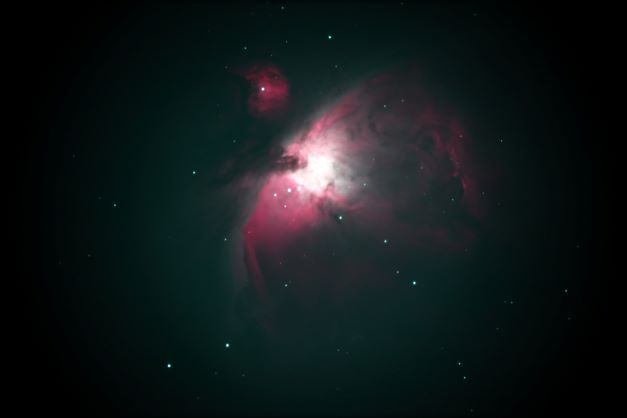
\includegraphics[width=\textwidth * 5/10]{images/orion.JPG}

% Now \textit{this} is quite something. But wait, you realize that the image seems... slightly smaller than the original? Thankfully, we can rectify this with padding.
% \begin{enumerate}[(i)]
%     \item \textbf{[3 points]} Briefly describe at least three different types of padding required on output images post convolution.

%     \begin{mdframed}
%         TODO: Your answer for (c) (i) here
%     \end{mdframed}

%     \begin{mdframed}[hidealllines=true,backgroundcolor=yellow]
%     \item \textbf{[1 point]} (Bonus) What kind of padding would you use on your image of the Orion Nebula? (There's no right answer, but please justify!)
%     \end{mdframed}
    
%     \begin{mdframed}
%         TODO: Your answer for (c) (ii) here
%     \end{mdframed}
% \end{enumerate}
\item \textbf{[5 points]} 
\begin{tcolorbox}[colback=orange!5!white,colframe=orange!75!black]
Why is image convolution important in Computer Vision? Which applications does it allow? (5-10 sentences)
\end{tcolorbox}
\end{enumerate}


% %%%%%%%%%%%%%%%%%%%%%%%%%%%%%%%%%%%
% \pagebreak
% \paragraph{A3:} Your answer here.
% % Uncomment the stencil below and fill in your solution.

% \begin{enumerate}[(a)]
% \item
% \begin{enumerate}[(i)]
%     \item
%     \begin{mdframed}
%         TODO: Your answer for (a) (i) here
%     }}
%     \item
%     \begin{mdframed}
%         TODO: Your answer for (a) (ii) here
%     }}
%     \item
%     \begin{mdframed}
%         TODO: Your answer for (a) (iii) here
%     }}
% \end{enumerate}
% \item
% \item
% \begin{enumerate}[(i)]
%     \item
%     \item (Bonus)
% \end{enumerate}
% \end{enumerate}

% %%%%%%%%%%%%%%%%%%%%%%%%%%%%%%%%%%%

% Please leave the pagebreak
\pagebreak
\paragraph{Q4:} \textbf{[8 points]} Now that you've successfully used convolution to de-noise your image of the Orion nebula, you decide to explore the filtering technique more closely. 

Specifically, you know two filtering operations exist: correlation and convolution. Both techniques extract (or delete) information from images.

\begin{enumerate}[(a)]
    \item \textbf{[2 points]} 
    \begin{tcolorbox}[colback=orange!5!white,colframe=orange!75!black]
    Comment on the difference between convolution and correlation, including their properties. 
    \end{tcolorbox}
    
    \begin{tcolorbox}[colback=white!5!white,colframe=green!75!black]
    \begin{mdframed}
        TODO: Your answer for (a) here
    \end{mdframed}
\end{tcolorbox}
    

    \item \textbf{[1 + 1 points]} 
    \begin{tcolorbox}[colback=orange!5!white,colframe=orange!75!black]
    You attempt to use both correlation and convolution on the mean filter over the orion nebula. Do you expect different output images? Generally, when do correlation and convolution produce identical results? (3-5 sentences)
    \end{tcolorbox}
    
    \begin{tcolorbox}[colback=white!5!white,colframe=green!75!black]
    \begin{mdframed}
        TODO: Your answer for (b) here
    \end{mdframed}
\end{tcolorbox}

    \item \textbf{[2 + 2 points]}
    You decide to solidify your understanding of the distinction between correlation and convolution by taking another image.
    
    \begin{tcolorbox}[colback=orange!5!white,colframe=orange!75!black]
    For this, come up with a use case where the output of correlation and convolution differ.
    
    Write some code that takes an image and produces two distinct images, one from convolution and one from correlation on some kernel of your choice. 
    
    Specify your kernel, and provide the input image and output results. Then, use your understanding of convolution and correlation to explain the outputs. (5-10 sentences)
    \end{tcolorbox}
    
    \emph{Please use \href{https://docs.scipy.org/doc/scipy/reference/generated/scipy.ndimage.convolve.html}{$scipy.ndimage.convolve$} and \href{https://docs.scipy.org/doc/scipy/reference/generated/scipy.ndimage.correlate.html}{$scipy.ndimage.correlate$} to experiment!}
    

\begin{tcolorbox}[colback=white!5!white,colframe=green!75!black]
    \includegraphics[width=\textwidth * 5/10]{TODO: original-img.png}\\
    \includegraphics[width=\textwidth * 5/10]{TODO: convolved-img.png}
    \includegraphics[width=\textwidth * 5/10]{TODO: correlated-img.png}
    
    \begin{mdframed}
        TODO: Your answer for (c) here
    \end{mdframed}
\end{tcolorbox}

\end{enumerate}


% %%%%%%%%%%%%%%%%%%%%%%%%%%%%%%%%%%%
% \paragraph{A4:} Your answer here.
% % Uncomment the stencil below and fill in your solution.

% \begin{enumerate}[(a)]
% \item
% \item
% \item
% \end{enumerate}

% %%%%%%%%%%%%%%%%%%%%%%%%%%%%%%%%%%%

% Please leave the page break
\pagebreak

\paragraph{Q5:} \textbf{[9 points]} You're a restoration architect who's in charge of determining when heritage site structures need a bit of upkeeping due to weather, erosion or other factors (natural and tourism-caused). This week, you've been assigned to visit a castle on a beautiful seafront to see if any restoration is in order.

After a heavy analysis, you decide the castle is in decent shape. As such, you need to convince your superior, so you snap a picture of the castle with your camera:

\includegraphics[width=\textwidth * 5/10]{images/castle.jpg}


%%%%%%%%%%%%%%%%%%%%%%%%%%%%%%%%%%%

% \emph{LaTeX:} To fill in boxes, replace `\textbackslash square' with `\textbackslash blacksquare' for your answer.

\begin{enumerate}[(a)]
\item \textbf{[2 points]} Oh no! Looks like there are some weird artefacts on the image, almost as though the walls are bleeding color? 
    
    \begin{tcolorbox}[colback=orange!5!white,colframe=orange!75!black]
This phenomena is called aliasing, but why has it happened?
\end{tcolorbox}
\begin{tcolorbox}[colback=white!5!white,colframe=green!75!black]
\begin{mdframed}
    TODO: Your answer for (a) here
\end{mdframed}
\end{tcolorbox}

\item \textbf{[3 points]}
You decide to fix this by passing your image through an anti-aliaser online. Amongst a host of complicated things, the software reduces the 'choppiness' of the image using low-pass filter convolution (some related high-pass filters also exist):

\includegraphics[width=\textwidth * 5/10]{images/castle-after.jpg}

\begin{tcolorbox}[colback=orange!5!white,colframe=orange!75!black]
Let's make sure we fully understand how this works though. Can you identify which of the following filters is high pass or low pass?
\end{tcolorbox}

\begin{enumerate}[(i)]
\item
 $\begin{bmatrix}
    1 & 0 & -1 \\
    1 & 0 & -1 \\
    1 & 0 & -1 \\
 \end{bmatrix}$
\begin{tcolorbox}[colback=white!5!white,colframe=green!75!black]
TODO: Select the appropriate answer.

\begin{tabular}[h]{ll}
$\square$ & High pass \\
$\square$ & Low pass \\
$\square$ & Neither \\
\end{tabular}
\end{tcolorbox}

\item
 $\begin{bmatrix}
    \frac{1}{9} & \frac{1}{9} & \frac{1}{9} \\
    \frac{1}{9} & \frac{1}{9} & \frac{1}{9} \\
    \frac{1}{9} & \frac{1}{9} & \frac{1}{9}
 \end{bmatrix}$
 \begin{tcolorbox}[colback=white!5!white,colframe=green!75!black]
TODO: Select the appropriate answer.

\begin{tabular}[h]{ll}
$\square$ & High pass \\
$\square$ & Low pass \\
$\square$ & Neither \\
\end{tabular}
\end{tcolorbox}

\item
$\begin{bmatrix}
    -\frac{1}{9} & -\frac{1}{9} & -\frac{1}{9} \\
    -\frac{1}{9} & \frac{8}{9} & -\frac{1}{9} \\
    -\frac{1}{9} & -\frac{1}{9} & -\frac{1}{9}
  \end{bmatrix}$
  \begin{tcolorbox}[colback=white!5!white,colframe=green!75!black]
TODO: Select the appropriate answer.

\begin{tabular}[h]{ll}
$\square$ & High pass \\
$\square$ & Low pass \\
$\square$ & Neither \\
\end{tabular}
\end{tcolorbox}
\end{enumerate}

\item \textbf{[2 points]}
You think you've gotten a full understanding of how the filters classify, but decide to test if you can recognize which filter has been used to get a target output image. 

\begin{tcolorbox}[colback=orange!5!white,colframe=orange!75!black]
Given the input image below, identify the filter that has been applied.
\end{tcolorbox}

\raisebox{\baselineskip-\height}{\includegraphics[width=\textwidth * 5/10]{images/q3img0.png}}

\begin{enumerate}[(i)]
\item
Output image 1:\\
\raisebox{\baselineskip-\height}{\includegraphics[width=\textwidth * 5/10]{images/q3img1.png}}
\begin{tcolorbox}[colback=white!5!white,colframe=green!75!black]
TODO: Select the appropriate answer.

\begin{tabular}[h]{lc}
$\square$ & High pass \\
$\square$ & Low pass \\
\end{tabular}
\end{tcolorbox}

\item
Output image 2:\\
\raisebox{\baselineskip-\height}{\includegraphics[width=\textwidth * 5/10]{images/q3img2.png}}
\begin{tcolorbox}[colback=white!5!white,colframe=green!75!black]
TODO: Select the appropriate answer.

\begin{tabular}[h]{lc}
$\square$ & High pass \\
$\square$ & Low pass \\
\end{tabular}
\end{tcolorbox}
\end{enumerate}

\item \textbf{[2 points]}
\begin{tcolorbox}[colback=orange!5!white,colframe=orange!75!black]
Which of the following statements are true? (Check all that apply).
\end{tcolorbox}

\begin{tcolorbox}[colback=white!5!white,colframe=green!75!black]
TODO: Select all that apply.

\begin{tabular}[h]{ll}
$\square$ & High pass filter kernels will always contain at least one negative number \\
$\square$ & A Gaussian filter is an example of a low pass filter \\
$\square$ & A high pass filter is the basis for most smoothing methods \\
$\square$ & In a high pass filter, the center of the kernel must have the highest value \\
\end{tabular}
\end{tcolorbox}

\end{enumerate}



%%%%%%%%%%%%%%%%%%%%%%%%%%%%%%%%%%%

% Please leave the pagebreak
\pagebreak
\paragraph{Q6:} \textbf{[7 points]}
    It is very important to understand how convolution/correlation scale with input size. A good measure of scale is measuring how the computation times of such filtering operations varies with filter sizes.
    
    To make an accurate assessment on this computational scaling, we will be using filters with dimensions $n \times n$ where $n$ is an odd number and $n \in [3, 15]$ (i.e. $3\times3$, $5\times5$, $7\times7$, etc.), and images of sizes between 0.25 to 8 megapixels.

\begin{enumerate}[(a)]
\item
    \textbf{[3 points]}
    \begin{tcolorbox}[colback=orange!5!white,colframe=orange!75!black]
    Complete the stencil code below to create a graph with one trace per filter size, where the x-axis represents the correlation/convolution between an image size, and y-axis represents the time to convolve/correlate that image.

    The stencil code imports the libraries you will need, but to understand how to use them, please look at the documentation.
    
    \begin{itemize}
    \item convolve/correlate - \href{https://docs.scipy.org/doc/scipy/reference/generated/scipy.ndimage.convolve.html}{$scipy.ndimage.convolve$} or \href{https://docs.scipy.org/doc/scipy/reference/generated/scipy.ndimage.correlate.html}{$scipy.ndimage.correlate$}
    \item rescale - \href{https://scikit-image.org/docs/dev/api/skimage.transform.html#skimage.transform.rescale}{$skimage.transform.rescale$}
    \item resize - \href{https://scikit-image.org/docs/dev/api/skimage.transform.html#skimage.transform.resize}{$skimage.transform.resize$}
    \item rescale vs resize – an example \href{http://scikit-image.org/docs/dev/auto_examples/transform/plot_rescale.html}{here}
    \end{itemize}
    
    \end{tcolorbox}

\emph{Note A megapixel is 1,048,576 ($2^{20}$) pixels (1024$\times$1024), or sometimes also 1,000,000 pixels (especially if you manufacture cameras). Megapixels is often shortened to MP or MPix.}

\emph{Image:} \href{RISDance.jpg}{RISDance.jpg} (in the .tex directory).

\begin{tcolorbox}[enhanced jigsaw,breakable,pad at break*=1mm,colback=white!5!white,colframe=green!75!black]
\begin{python}
import time
import matplotlib.pyplot as plt
from skimage import io, img_as_float32
#use to rescale+resize image
from skimage.transform import rescale, resize
#use to convolve/correlate image
from scipy.ndimage import correlate

#This reads in image and converts to a floating point format
# 1) TODO - replace PATH with the actual path to the
#    downloaded RISDance.jpg image linked above
image = img_as_float32(io.imread('PATH'))

# 2) TODO - change the image size so it starts
#    at 8MPix (calculated as height x width)
#    use one of the imported libraries
original_image =

# 3) TODO - iterate through odd numbers from 3 to 15
#   (inclusive!!) these will represent your filter sizes
#   (3x3,5x5,7x7, etc.), for each filter size you will...
for kernel_size in range():

    #because for each loop you are resizing your image, you
    #want to start each loop w/the original image size
    shrinking_image = original_image

    #these lists will hold the values you plot
    image_sizes = [] #x axis
    times = [] #y axis

    #while image size is bigger than .25MPx
    while(shrinking_image.size > 250000):

    	# 4) TODO - create your kernel. Your kernel can hold
    	#    any values, as the kernel values shouldn't
    	#    affect computation time. Avoid using np.zeros to
    	#    create your kernal, as this messes up the intended
    	#    output graph. The size of the kernel
    	#    must be kernel_size x kernel_size
        kernel =

        #5) TODO - reduce your image size. You can choose by
        # what increments to reduce your image.
        shrinking_image =

        #gets the current time (in seconds)
        start = time.time()

        # 6) TODO - use one of the imported libraries to do
        # your correlation/convolution on the image. You can
        # choose which operation to perform.


        #gets the current time (in seconds)
        end = time.time()

        #7) TODO - figure out what values to append, and
        #   append them here
        image_sizes.append()
        times.append()

    #each filter size will be plotted as a separate line, in
    #a multi-line 2-dimensional graph
    plt.plot(image_sizes, times, label=str(kernel.size))

#plot
plt.xlabel('image size (pixels)')
plt.ylabel('operation time (seconds)')
plt.legend(title="filter sizes (pixels)")
plt.show()

\end{python}
\end{tcolorbox}
    
    
    \item \textbf{[2 points]}
    \begin{tcolorbox}[colback=orange!5!white,colframe=orange!75!black]
    Present your graph with a brief description of what your graph demonstrates.
    \end{tcolorbox}

\begin{tcolorbox}[colback=white!5!white,colframe=green!75!black]
    \begin{mdframed}
        TODO: Your answer for (a) (ii) here
    \end{mdframed}
\end{tcolorbox}
    

\item \textbf{[2 points]} 
\begin{tcolorbox}[colback=orange!5!white,colframe=orange!75!black]
Do the results match your expectation given the number of multiply and add operations in convolution? (3-5 sentences)
\end{tcolorbox}
    
    \begin{tcolorbox}[colback=white!5!white,colframe=green!75!black]
    \begin{mdframed}
        TODO: Your answer for (b) here
    \end{mdframed}
\end{tcolorbox}
    
\end{enumerate}

% %%%%%%%%%%%%%%%%%%%%%%%%%%%%%%%%%%%
% \pagebreak
% \paragraph{A6:} Your graph and answer here.
% % Uncomment the stencil below and fill in your solution.

% % \begin{enumerate}[(a)]

% % \item Add your graph as well as a brief description of what your graph demonstrates.

% % \item Do the results match your expectation given the number of multiply and add operations in convolution?

% % \end{enumerate}

% %%%%%%%%%%%%%%%%%%%%%%%%%%%%%%%%%%%
\pagebreak
\paragraph{Q7:} \textbf{[7 points]} The \texttt{numpy} library is extremely important when working with input data (vectors or matrices) and their linear algebra manipulations. In Computer Vision, your data will often come in the form of matrices of images (pixel representations). 

 To familiarize yourself with the library, read through the following scenarios and complete the exercises. Write \emph{one} \texttt{numpy} function to complete each of the following tasks.

Note that numpy is usually imported as
\begin{verbatim}
    import numpy as np
\end{verbatim}
at the top of the code file. You can then call numpy functions with \begin{verbatim}
    np.function_name(<arguments>)
\end{verbatim}
You are encouraged to test out your answers by creating your own python program, importing numpy and calling and printing the results of your solutions! Some numpy functions you might find useful are \href{https://numpy.org/doc/stable/reference/generated/numpy.squeeze.html}{np.squeeze}, \href{https://numpy.org/doc/stable/reference/generated/numpy.expand_dims.html}{np.expand\_dims}, \href{https://numpy.org/doc/stable/reference/generated/numpy.clip.html}{np.clip}, \href{https://numpy.org/doc/stable/reference/generated/numpy.pad.html}{np.pad}, and \href{https://numpy.org/doc/stable/reference/generated/numpy.zeros.html}{np.zeros}.

You may also use operators like \texttt{[]} and \texttt{:}, but remember to use only \textit{one} function/operator shorthand.

\begin{enumerate}[(a)]
    \item \textbf{[1 point]} You're attempting to create a black image base, \texttt{img}. All values in this matrix are 0. 
    
    \begin{tcolorbox}[colback=orange!5!white,colframe=orange!75!black]
    Create \texttt{img} where \texttt{np.shape(img) == (320,640)}.
    \end{tcolorbox}
    
    \begin{tcolorbox}[colback=white!5!white,colframe=green!75!black]
    \begin{mdframed}
        TODO: Your answer for (a) here
    \end{mdframed}
\end{tcolorbox}
    
    \item \textbf{[1 point]} You've been working on a Computer Vision pipeline that de-noises your image. Unfortunately, it seems to mess up the dimensions, and outputs an image-array, \texttt{img\_out}, where \texttt{np.shape(img\_out) == (1, 1, 320, 640)}. 
    
    \begin{tcolorbox}[colback=orange!5!white,colframe=orange!75!black]
    Convert \texttt{img\_out} to a new 2D image-array, \texttt{img\_fixed}, where \texttt{np.shape(img\_fixed) == (320, 640)}. In other words, remove all the 1-sized dimensions.
    \end{tcolorbox}

\begin{tcolorbox}[colback=white!5!white,colframe=green!75!black]
    \begin{mdframed}
        TODO: Your answer for (b) here
    \end{mdframed}
\end{tcolorbox}
    
    \item \textbf{[1 point]} Usually, image-arrays are represented with three dimensions. The first dimension represents the number of channels, and can be used to identify if an image is RGB or grayscale. 
    
    \begin{tcolorbox}[colback=orange!5!white,colframe=orange!75!black]
    Say you have a grayscale image-array \texttt{img} where \texttt{np.shape(img) == (320, 640)}. Convert this to a new image-array, \texttt{img\_expanded}, which appropriately captures the number of channels, where \texttt{np.shape(img\_expanded) == (1, 320, 640)}. In other words, add a dimension to \texttt{img}.
    \end{tcolorbox}

\begin{tcolorbox}[colback=white!5!white,colframe=green!75!black]
    \begin{mdframed}
        TODO: Your answer for (c) here
    \end{mdframed}
\end{tcolorbox}
    
    \item \textbf{[1 point]} When you learn about Convolutional Neural Networks later in the course, you'll find yourself needing to normalize input images such that each channel has intensities ranging from -1 to 1 instead of 0 to 255.
    
    \begin{tcolorbox}[colback=orange!5!white,colframe=orange!75!black]
    Assume you have a linearly normalized grayscale 2D image-array, \texttt{img} (the channel dimension of 1 has already been removed), and want to remove outlier intensities and artefacts (such as glare). Clip \texttt{img} so all its values lie within the range [-0.5, 0.5].
    \end{tcolorbox}

\begin{tcolorbox}[colback=white!5!white,colframe=green!75!black]
    \begin{mdframed}
        TODO: Your answer for (d) here
    \end{mdframed}
\end{tcolorbox}
    
    \item \textbf{[1 point]} Let's say you're trying to code a red-green-filter function. This will take in an RGB image-array, \texttt{img}, (this means the image has 3 channels), and filters all but the blue channel. Note that \texttt{np.shape(img) == (320, 640, 3)}.
    
    \begin{tcolorbox}[colback=orange!5!white,colframe=orange!75!black]
    Retrieve the blue channel of \texttt{img} while preserving all of \texttt{img}'s dimensions and intensity values.
    \end{tcolorbox}
    
    \begin{tcolorbox}[colback=white!5!white,colframe=green!75!black]
    \begin{mdframed}
        TODO: Your answer for (e) here
    \end{mdframed}
\end{tcolorbox}
    
    \item \textbf{[1 point]} Let's say you're trying to code a green-filter function. This will take in an RGB image-array, \texttt{img}, and filters out the green channel. Note that \texttt{np.shape(img) == (320, 640, 3)}. 
    
    \begin{tcolorbox}[colback=orange!5!white,colframe=orange!75!black]
    Retrieve the red and blue channels of \texttt{img} while preserving all of \texttt{img}'s dimensions and intensity values.
    \end{tcolorbox}
    
    \begin{tcolorbox}[colback=white!5!white,colframe=green!75!black]
    \begin{mdframed}
        TODO: Your answer for (f) here
    \end{mdframed}
\end{tcolorbox}
    
    \item \textbf{[1 point]} Same-Padding is a useful tool to ensure that the dimensions of the output image from a convolution operation matches the dimensions of the input image. 
    
    \begin{tcolorbox}[colback=orange!5!white,colframe=orange!75!black]
    Given an RGB image-array, \texttt{img}, pad it with two columns of zeros on the left and right edges of the image, and three rows of zeros on the top and bottom edges of the image. Don't add zeros to the color channel dimension (the front and back faces of the image-array).
    \end{tcolorbox}
    
    \begin{tcolorbox}[colback=white!5!white,colframe=green!75!black]
    \begin{mdframed}
        TODO: Your answer for (g) here
    \end{mdframed}
\end{tcolorbox}
    
\end{enumerate}


% %%%%%%%%%%%%%%%%%%%%%%%%%%%%%%%%%%%
% \pagebreak
% \paragraph{A7:} Your answer here. Remember, write \emph{one} numpy function to complete each of the tasks---this includes operators like [] and :.
% %  Uncomment the stencil below and fill in your solution.

% % \begin{enumerate}[(a)]
% % \item
% % \item
% % \item
% % \item
% % \item
% % \item
% % \item
% % \end{enumerate}


% %%%%%%%%%%%%%%%%%%%%%%%%%%%%%%%%%%%
% Please leave the pagebreak
%% any suggestions for more?
\pagebreak
\section*{Feedback? (Optional)}
Please help us make the course better. If you have any feedback for this assignment, we'd love to hear it!

\end{document}
